
\documentclass[tikz,border=8pt]{standalone}
\usepackage{amsmath}
\begin{document}
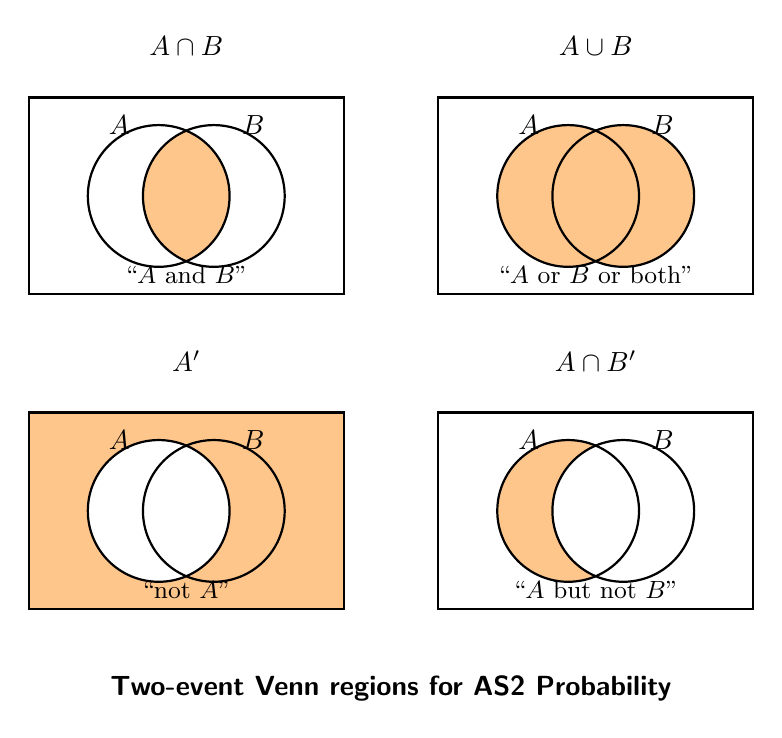
\begin{tikzpicture}[font=\sffamily,venncircle/.style={draw=black,line width=0.8pt},samplebox/.style={draw=black,line width=0.8pt},shade/.style={fill=orange!45,draw=none},title/.style={font=\sffamily\bfseries}]
\begin{scope}[shift={(0,0)}]
\node[title] at (2,3.15) {$A\cap B$}; \draw[samplebox] (0,0) rectangle (4,2.5); \begin{scope}\clip (1.65,1.25) circle (0.9); \fill[shade] (2.35,1.25) circle (0.9);\end{scope}\draw[venncircle] (1.65,1.25) circle (0.9);\draw[venncircle] (2.35,1.25) circle (0.9);\node at (1.15,2.15) {$A$};\node at (2.85,2.15) {$B$};\node[font=\small] at (2,0.25) {``$A$ and $B$''};
\end{scope}
\begin{scope}[shift={(5.2,0)}]
\node[title] at (2,3.15) {$A\cup B$}; \draw[samplebox] (0,0) rectangle (4,2.5); \fill[shade] (1.65,1.25) circle (0.9);\fill[shade] (2.35,1.25) circle (0.9);\draw[venncircle] (1.65,1.25) circle (0.9);\draw[venncircle] (2.35,1.25) circle (0.9);\node at (1.15,2.15) {$A$};\node at (2.85,2.15) {$B$};\node[font=\small] at (2,0.25) {``$A$ or $B$ or both''};
\end{scope}
\begin{scope}[shift={(0,-4)}]
\node[title] at (2,3.15) {$A'$}; \fill[shade] (0,0) rectangle (4,2.5);\draw[samplebox] (0,0) rectangle (4,2.5);\fill[white] (1.65,1.25) circle (0.9);\draw[venncircle] (1.65,1.25) circle (0.9);\draw[venncircle] (2.35,1.25) circle (0.9);\node at (1.15,2.15) {$A$};\node at (2.85,2.15) {$B$};\node[font=\small] at (2,0.25) {``not $A$''};
\end{scope}
\begin{scope}[shift={(5.2,-4)}]
\node[title] at (2,3.15) {$A\cap B'$}; \draw[samplebox] (0,0) rectangle (4,2.5); \fill[shade] (1.65,1.25) circle (0.9);\fill[white] (2.35,1.25) circle (0.9);\draw[venncircle] (1.65,1.25) circle (0.9);\draw[venncircle] (2.35,1.25) circle (0.9);\node at (1.15,2.15) {$A$};\node at (2.85,2.15) {$B$};\node[font=\small] at (2,0.25) {``$A$ but not $B$''};
\end{scope}
\node[font=\sffamily\bfseries] at (4.6,-5.0) {Two-event Venn regions for AS2 Probability};
\end{tikzpicture}
\end{document}
